The system, named \textit{Miraihilate}, is a software program intended to be used by system administrators to scan their private network(s) to detect a vulnerability in Linux devices that Mirai malware exploits, and attempts to patch this vulnerability if it is found. It will enable users of the system to perform simple operations such as a quick scan on the network, as well as providing advanced scanning options and other utilities for the user.

\vspace{0.5cm}

The functionality of Miraihilate will be separated into two parts, the \textit{back-end} scripts and the \textit{front-end} client interface, as well as coming with a setup utility to setup the program with an initial administrator user.

\vspace{0.5cm}

As well as just the interface that the user interacts with, Miraihilate will also implement a secure role-based entry system as well as a logging system. Because of Miraihilate's potential to access IoT device root accounts to patch the vulnerability to Mirai malware, it is eseential to create a secure access control system as well as securing access/scan logs to prevent malicious activites such as:
\begin{itemize}
	\item{Unauthorised access of scanning utilities}
	\item{Unauthorised accessand reading of log files}
\end{itemize}

\subsection{User Access Control}

Before a user can access the system, they must login to access the features. The login functionality will use BCrypt for hasing passwords, which is a default password hashing algorithm for some Linux distributions, such as OpenBSD\textsuperscript{\cite{openbsdbcrypt}} and SUSE Linux.

\vspace{0.5cm}

It incorporates a salt to protect against rainbow tables and is also adaptive to remain resistant to brute-force attacks, by increasing the iteration count (work factor) to make it slower. When using a suitable work factor and a secure password, it is practically infeasible to try every possible combination to crack the password. For Miraihilate, I will use a work factor of 12 and passwords \textbf{must} contain at least one uppercase letter and a symbol.

\vspace{0.5cm}

The form of access control used in Miraihilate will be role-based access control, which will regulate the tasks that certain users can perform. For the initial version of the program, there will be two roles: operator and administrator. Operators will be able to perform all operations that an administrator can with the difference being they cannot read log files that are not their own, nor can they add and remove other users from Miraihilate.

\subsection{Log System}

There will be two types of logs recorded in the system, which are access and scan logs. Access logs will be stored with a timestamp of when a user has accessed the system, to help identify who was on the system in case a problem arises. Scan logs will contain the start and end timestamps of the scan, as well as raw data about the scan that has taken place such as who started the scan and the number of vulnerable devices found in a given network range.

\subsection{Database Structure}

Before working on the implementation, I prepared the the database by creating an ER diagram to describe its structure and key relations between the data. Below is the ER diagram for the database that Miraihilate will use:

\begin{figure}[h]
	\centering
	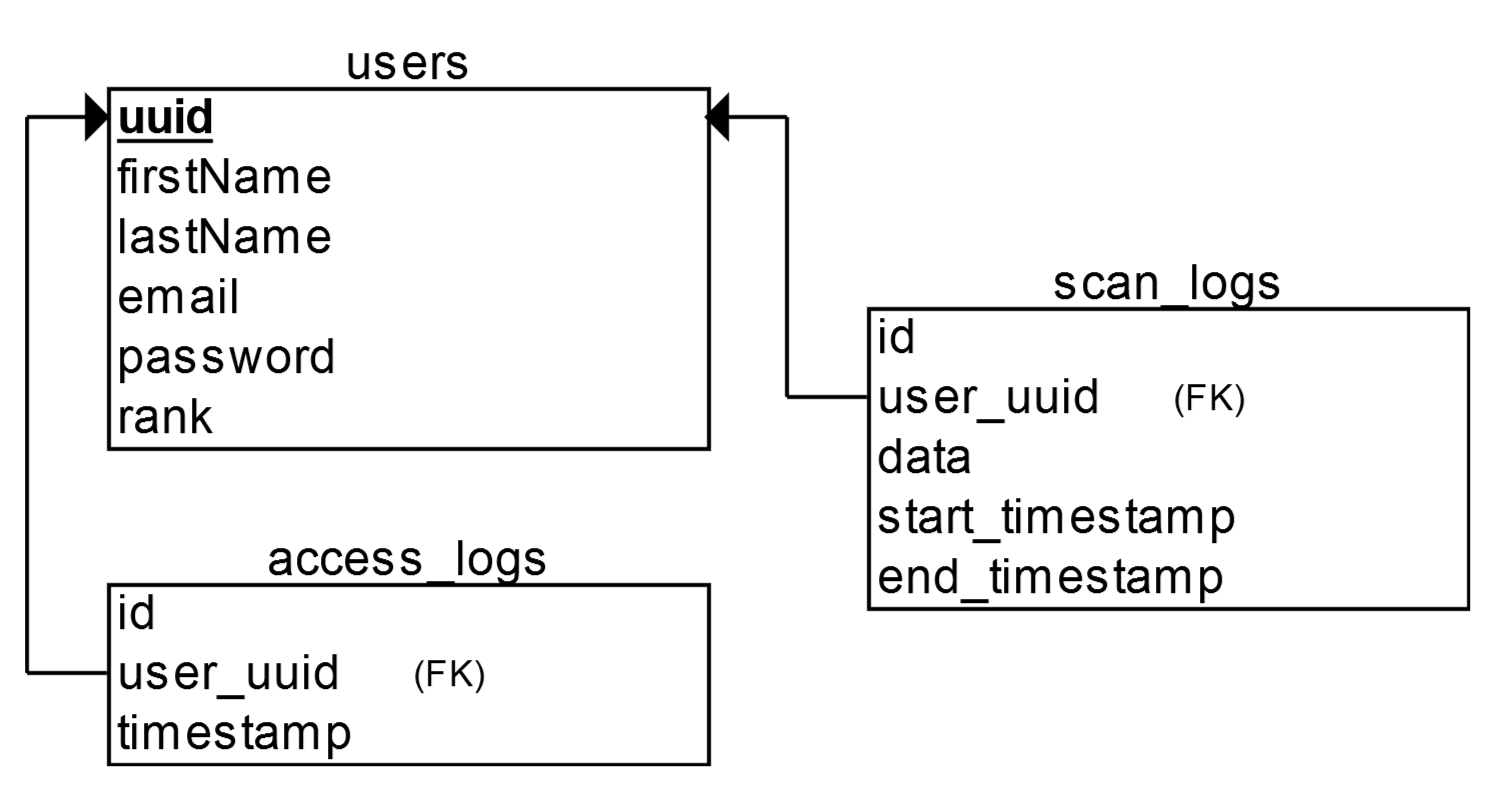
\includegraphics[width=0.75\linewidth]{img/miraihilate_erd_4x.png}
	\caption{Miraihilate Database ER Diagram}
\end{figure}

The \textit{data} field described in the above ER diagram will store raw HTML data, which will then be displayed in the HTML client. Since the database will not allow script tag characters, I will encase all disallowed characters with a backslash and then remove them upon retrieval in the client before being displayed.
